\section{Observations}
\label{sec:observations}

% 2394 = EDFS_comcam
% 5526 = Rubin_SV_095_-25
% 453 = 47Tuc
% 5063 = ECDFS
% 7611 = seagull
% 4016 = Fornax dSph
% 10463 = Rubin_SV_38_7

% 47 Tuc Globular Cluster (47 Tuc)
% (ra, dec) = (6.02, -72.08)

% Low Ecliptic Latitude Field (Rubin SV 38 7)
% (ra, dec) = (37.86, 6.98)

% Fornax Dwarf Spheroidal Galaxy (Fornax dSph)
% (ra, dec) = (40.00, -34.45)

% Extended Chandra Deep Field South (ECDFS)
% (ra, dec) = (53.13, -28.10)

% Euclid Deep Field South (EDFS)
% (ra, dec) = (59.10, -48.73)

% Low Galactic Latitude Field (Rubin SV 95 -25)
% (ra, dec) = (95.00, -25.00)

% Seagull Nebula (Seagull)
% (ra, dec) = (106.23, -10.51)

\begin{table*}
    \centering
    \begin{tabular}{@{}lcc@{}}
    \textbf{Field Name} & \textbf{RA} & \textbf{Declination} \\
     & \textit{deg} & \textit{deg} \\
    \hline
    47 Tuc Globular Cluster (47 Tuc)              & 6.02    & -72.08    \\
    Low Ecliptic Latitude Field (Rubin SV 38 7)   & 37.86   & 6.98      \\
    Fornax Dwarf Spheroidal Galaxy (Fornax dSph)  & 40.00   & -34.45    \\
    Extended Chandra Deep Field South (ECDFS)     & 53.13   & -28.10    \\
    Euclid Deep Field South (EDFS)                & 59.10   & -48.73    \\
    Low Galactic Latitude Field (Rubin SV 95 -25) & 95.00   & -25.00    \\
    Seagull Nebula (Seagull)                      & 106.23  & -10.51    \\
    \end{tabular}
    \caption{Seven target fields observed for Science Pipelines commissioning during the ComCam on-sky campaign.}
    \label{tab:target_fields}
\end{table*}


\begin{figure}
    \begin{center}
        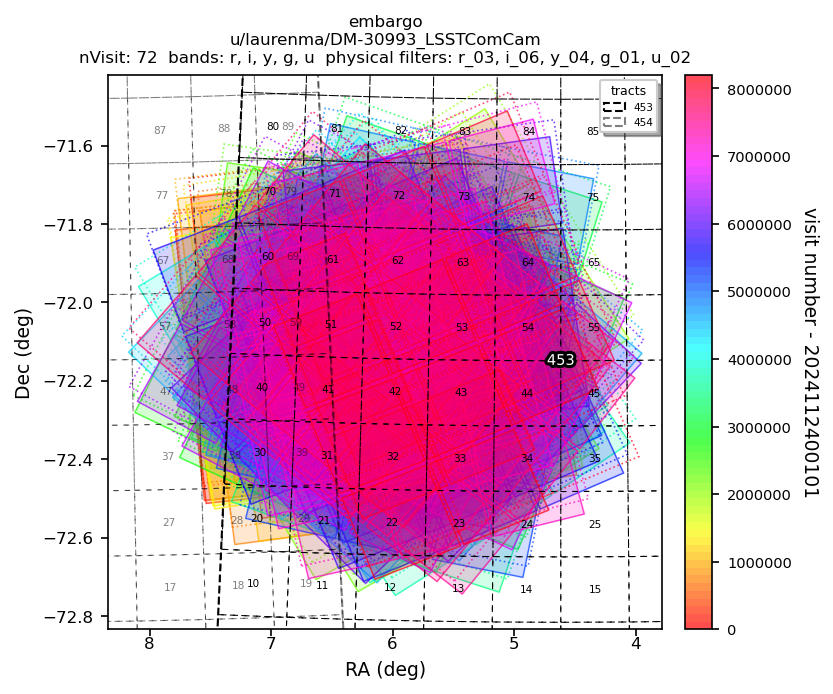
\includegraphics[width=0.3\textwidth]{observations_figures/showVisit_DM-30993_LSSTComCam_453.png}
        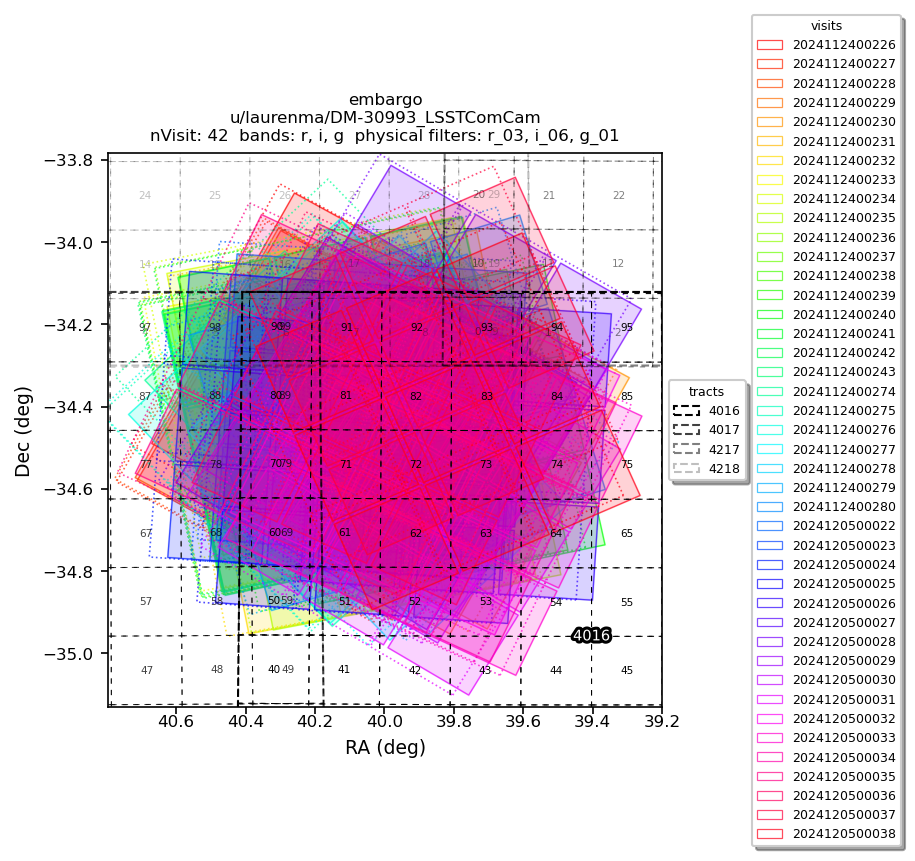
\includegraphics[width=0.3\textwidth]{observations_figures/showVisit_DM-30993_LSSTComCam_4016.png}
        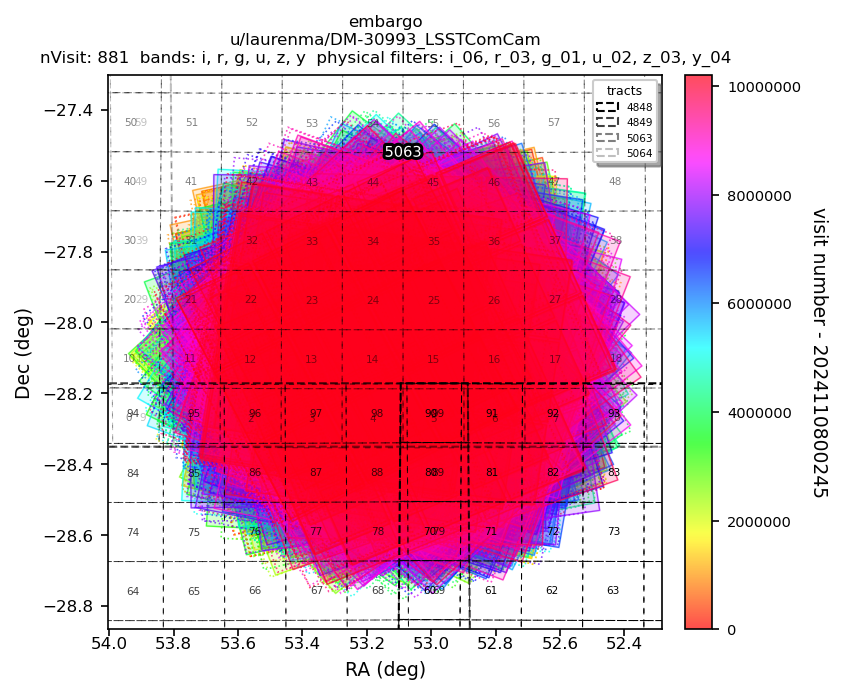
\includegraphics[width=0.3\textwidth]{observations_figures/showVisit_DM-30993_LSSTComCam_5063.png}
        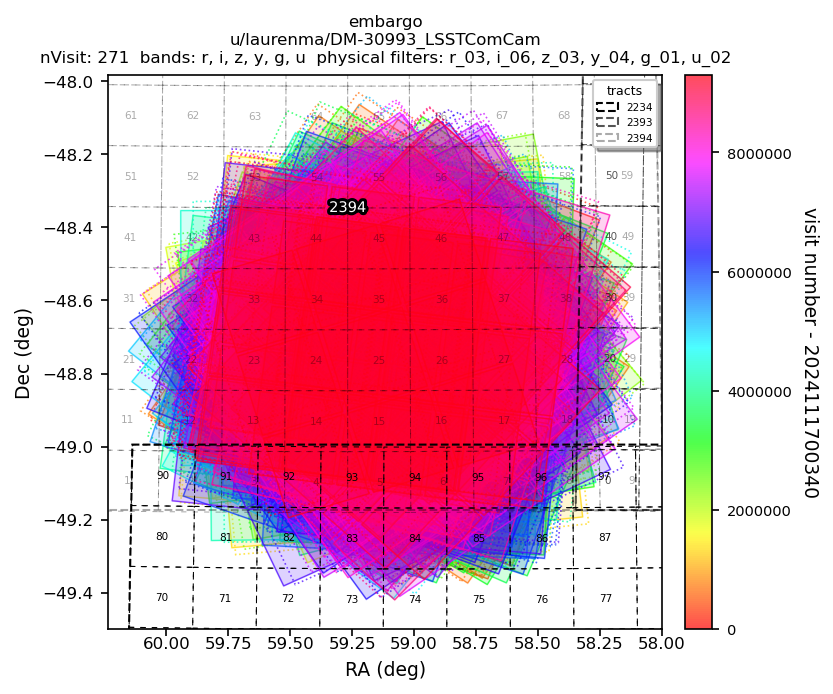
\includegraphics[width=0.3\textwidth]{observations_figures/showVisit_DM-30993_LSSTComCam_2394.png}
        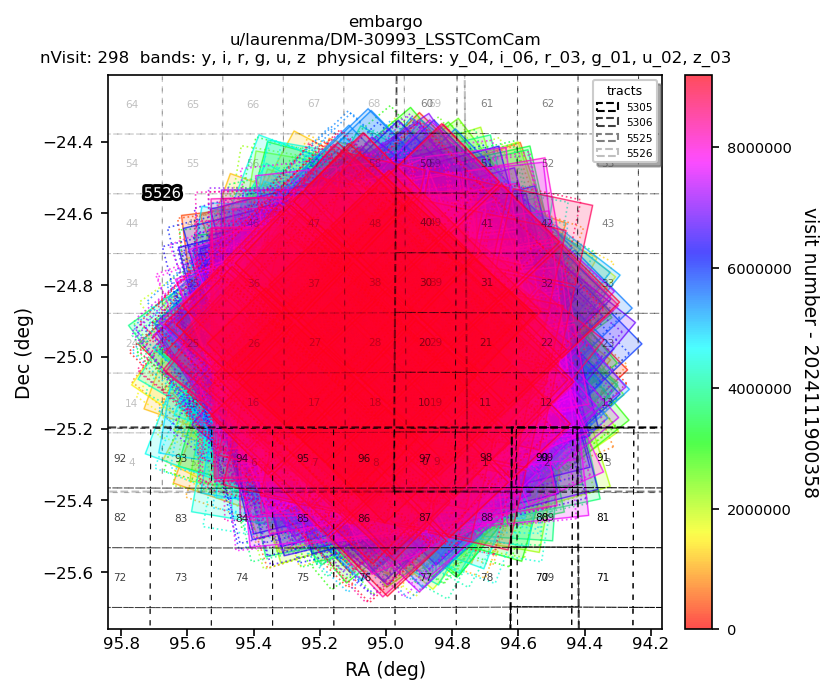
\includegraphics[width=0.3\textwidth]{observations_figures/showVisit_DM-30993_LSSTComCam_5526.png}
        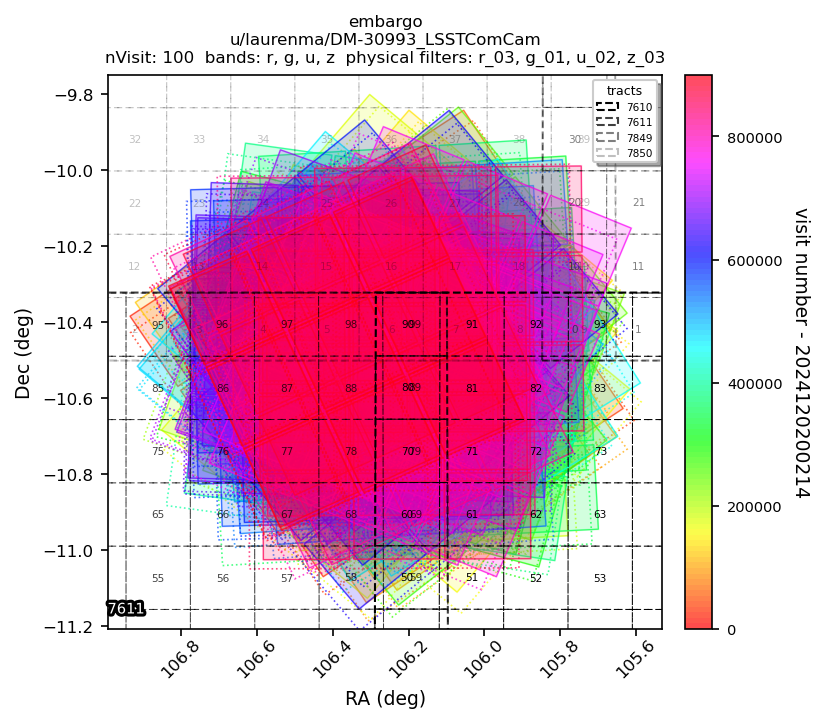
\includegraphics[width=0.3\textwidth]{observations_figures/showVisit_DM-30993_LSSTComCam_7611.png}
    \end{center}
    \caption{Sky coverage for six ComCam Deep Drilling Fields.
    First Row (left to right): 47 Tuc, Fornax dSph, ECDFS.
    Second Row (left to right): EDFS, RubinSV 95 -25, Seagull.}
    \label{fig:comcam_ddf_coverage}
\end{figure}

\begin{figure}
    \begin{center}
      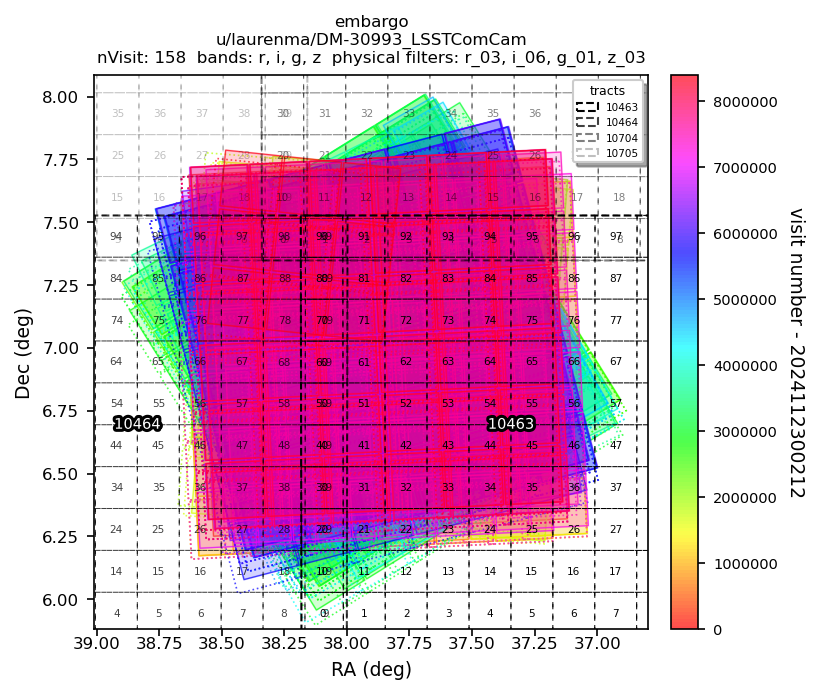
\includegraphics[width=0.3\textwidth]{observations_figures/showVisit_DM-30993_LSSTComCam_10463.png}
    \end{center}
    \caption{Sky coverage for Low Ecliptic Latitude Field (Rubin SV 38 7) during the ComCam on-sky campaign.}
    \label{fig:comcam_ecliptic_coverage}
\end{figure}